% !TeX encoding = UTF-8
\section{Einführung}

\begin{frame}{Einführung}
	\begin{minipage}[t][0.25\textheight]{1\textwidth}
		\centering
		\qq{I can't find an efficient algorithm, \\ but neither can all these famous people.} \\ --- \textit{Garey und Johnson} ---
	\end{minipage}
	\pause
	\begin{minipage}[t][0.5\textheight]{1\textwidth}
	\begin{itemize}
		\item Annahme für alle folgenden Überlegungen: NP $\neq$ P
		\item Ein Problem ist NP-schwer, wenn es keinen Algorithmus gibt, der
			\begin{itemize}
				\item	deterministisch,
				\item exakt für alle Eingaben und 
				\item	effizient für alle Eingaben arbeitet.
			\end{itemize}
		\end{itemize}
	\end{minipage}
\end{frame}

\begin{frame}{Auswege aus der NP-Vollständigkeit}
\begin{itemize}
	\item In der Praxis sind NP-vollständige Problem jedoch trotzdem gut lösbar
	\item Auflockerung der obigen Bedingungen
	\item Effizient für \st{alle} gewisse Eingaben 
	\begin{itemize}
		\item[] $\Rightarrow$ Pseudopolynomielle Algorithmen
	\end{itemize}
	\item \st{Exakte} Approximierte Lösung
	\begin{itemize}
		\item[] $\Rightarrow$ Polynomielle Approximationsschemata
	\end{itemize}
\end{itemize}
\end{frame}

\begin{frame}{\textsc{Rucksack}-Problem}
    \textsc{Rucksack} ist ein NP-vollständiges Problem \\~\\
    \pause
    Grundidee: \qq{Qual der Wahl}
    
    \begin{itemize}
        \item Ein Dieb raubt einen Laden aus, jedoch hat er für die Beute nur einen Rucksack dabei
        \item Im Laden findet er $n$ Gegenstände
        \item Der $i$-te Gegenstand hat den Wert $p_i$ und das Gewicht $w_i$
        \item Sein Rucksack kann höchstens das Gewicht $B$ tragen
        \item $p_i, w_i$ und $B$ sind natürliche Zahlen
    \end{itemize}
    \alert{Welche Gegenstände sollten für den maximalen Profit gewählt werden?} 
\end{frame}
\begin{frame}{Beispiel}
    \begin{figure}[ht]
    	\centering
    	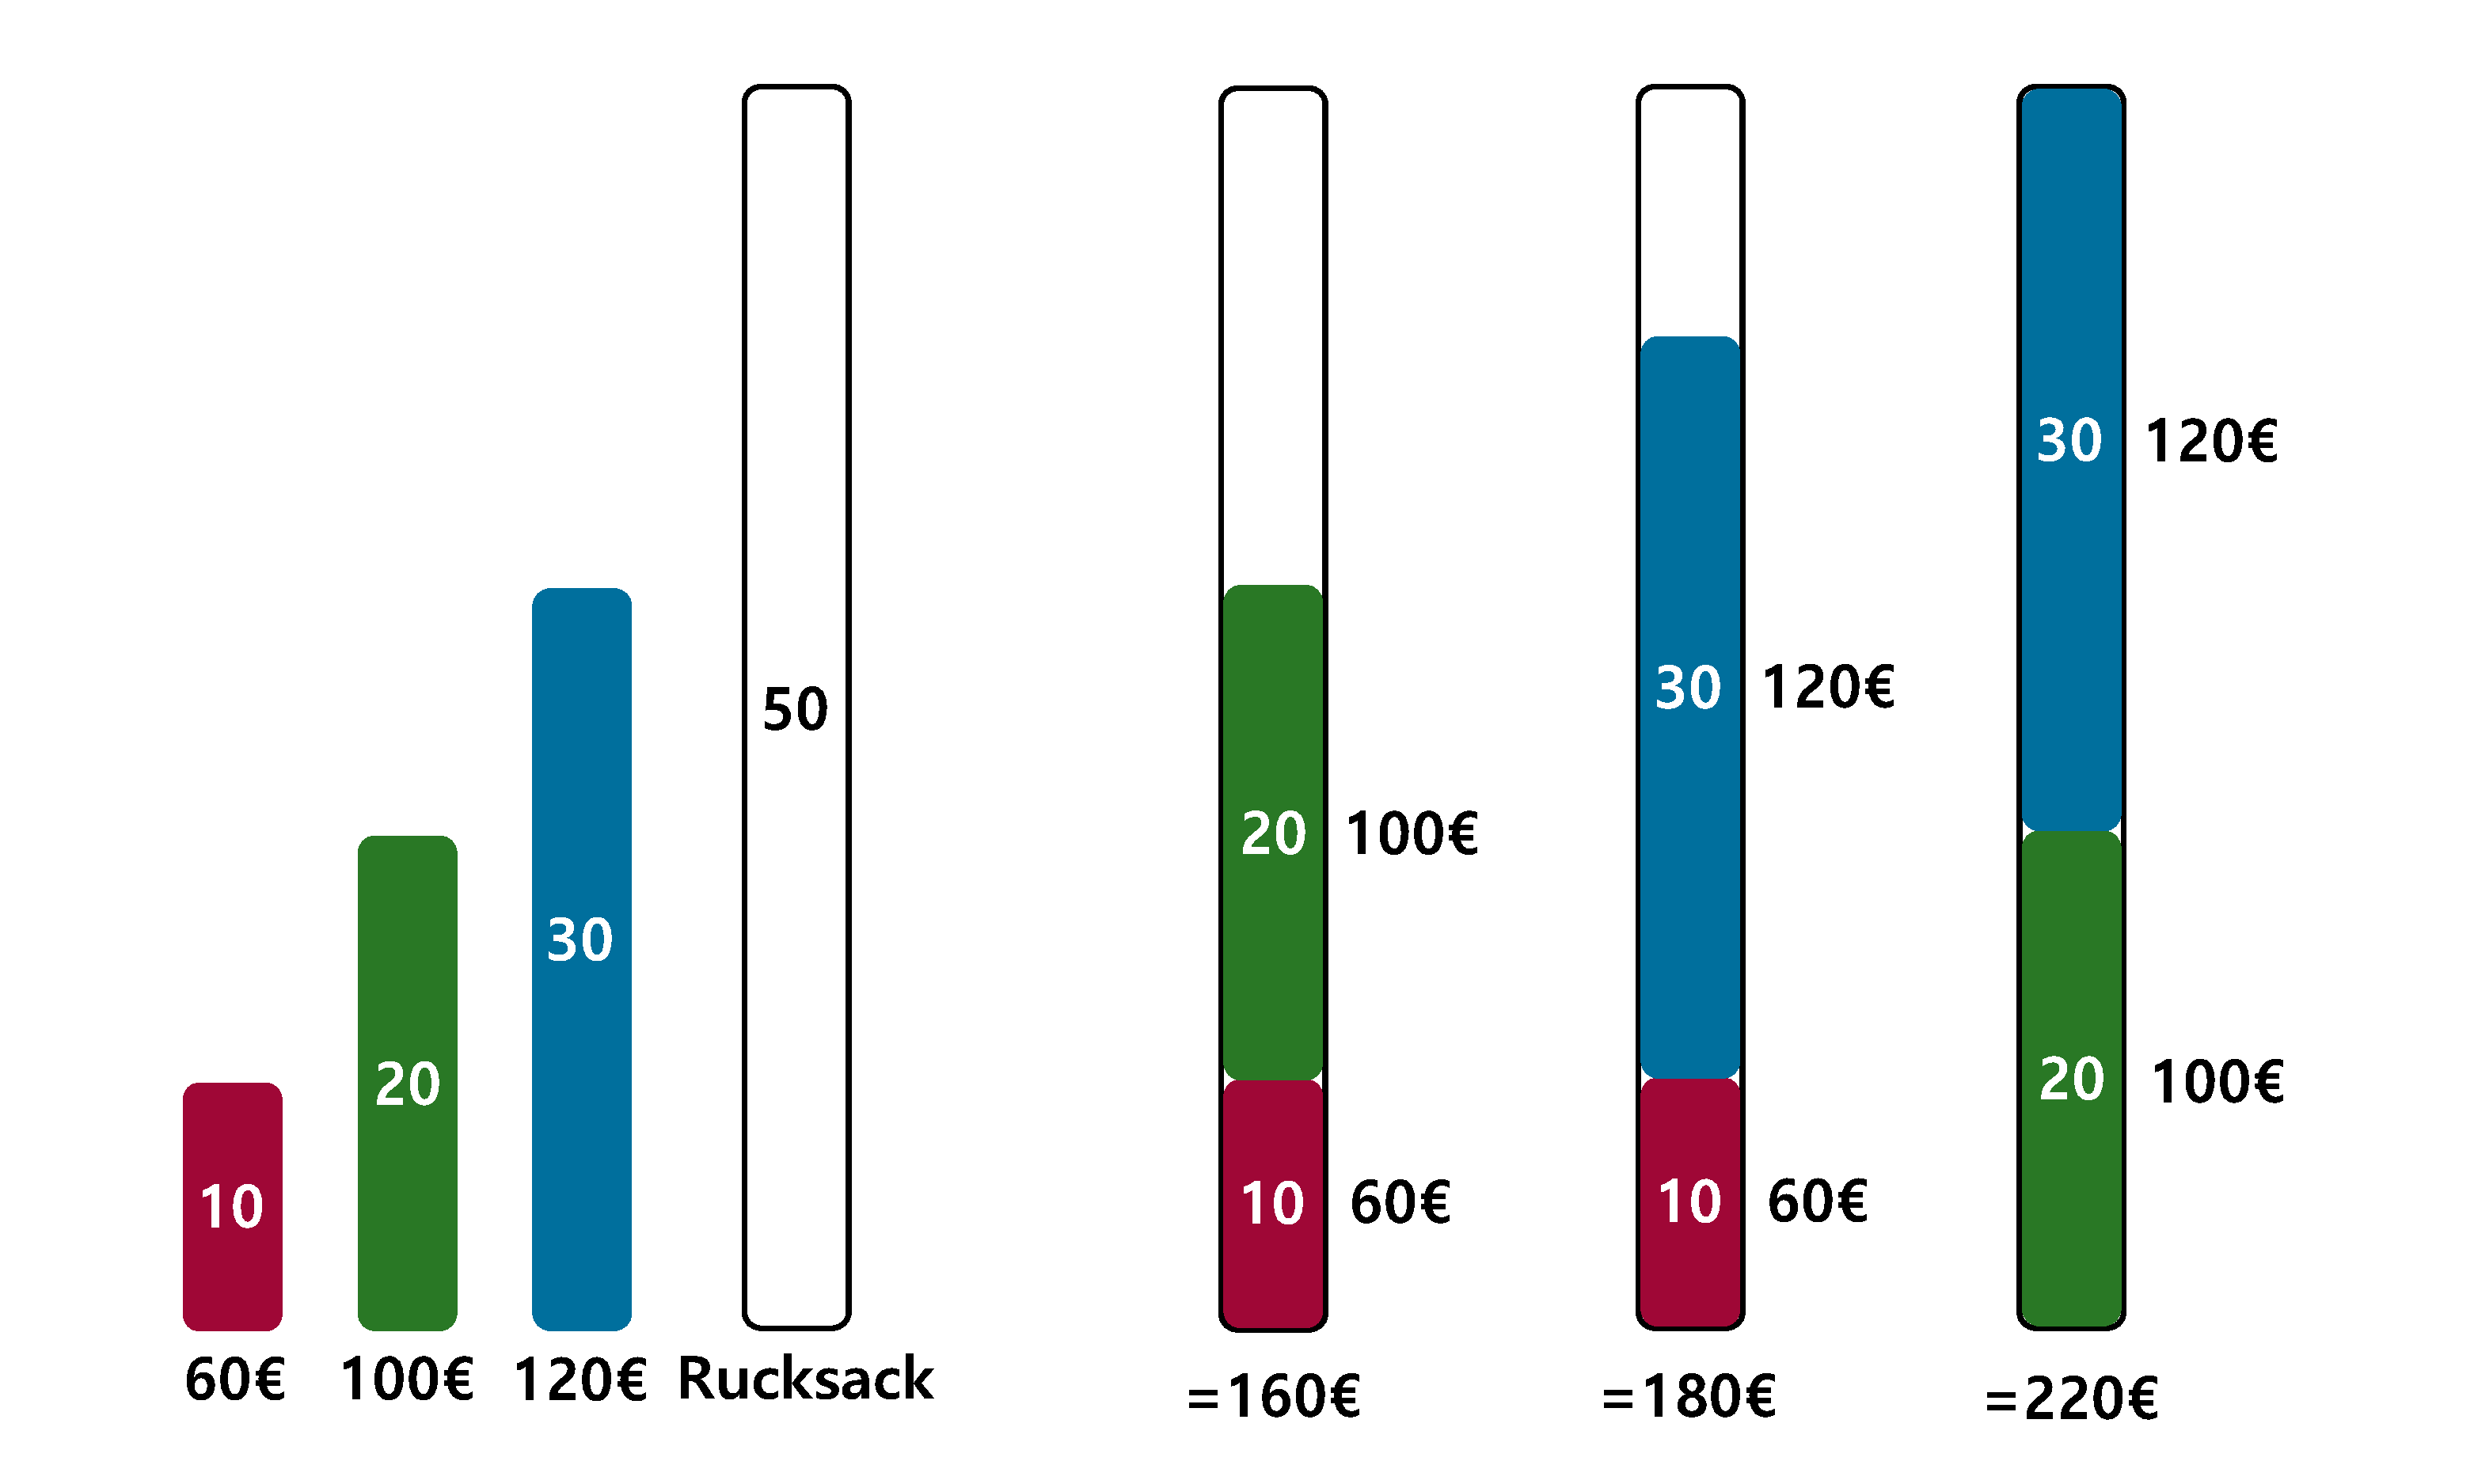
\includegraphics[width=0.9\textwidth]{img/Rucksack.pdf}
    	\caption{Rucksackproblem}
    	\label{fig:rucksack}
    \end{figure}
\end{frame}
\begin{frame}{\textsc{Rucksack}-Problem formal}
    \begin{itemize}
        \item $\begin{aligned}[t] \displaystyle
            \mathcal{D}=\{\langle W,w,p,B \rangle \mid & W=\{1,...,n\}, & \\
                                                                & w \colon W \to \mathbb{N}, & \\
                                                                & p \colon W \to \mathbb{N}, & \\
                                                                & B \in \mathbb{N}, & \\
                                                                & \forall i \in W \colon w_i \leq B\}
         \end{aligned}$
        
        \item $\displaystyle S( \langle W, w, p, B \rangle )=\{ A \subseteq W \mid \sum_{i\in A}{ w_i} \leq B \}$
        \item $\displaystyle f(A)=\sum_{i\in A}{p_i}$
        \item $\displaystyle \max$
    \end{itemize}
\end{frame}
\begin{frame}{0-1 \textsc{Rucksack}-Problem}
    maximiere $\displaystyle \sum_{i=1}^{n}{x_i p_i}$
       
    unter der Bedingung $\displaystyle \sum_{i=1}^{n}{x_i w_i \leq B}$
       
    mit $x_i=1$ wenn Gegenstand $i$ im Rucksack enthalten ist, sonst $x_i=0$
\end{frame}
\begin{frame}{0-1 \textsc{Rucksack}-Problem}
    Maximaler Profit ohne Überschreitung des Rucksackvolumen.
    Idee: Profit diskret erhöhen und prüfen ob mehr gehen würde.
    Hierzu benötigen wir eine Funktion die für einen bestimmten Wert $\alpha$ das minimal benötige Volumen zurück gibt.
    So können wir prüfen ob unser Rucksackvolumen $B$ bei einem bestimmten Profit $\alpha$ überschritten ist.
    Dynamische Lösung: Schritt für Schritt an die optimale Lösung heran arbeiten.
\end{frame}
\begin{frame}{0-1 \textsc{Rucksack}-Problem}
    Für $j \in \{0,1,...,n\}$ und $\alpha \in \mathbb{Z}$ sei $F_j(\alpha)$ das kleinste benötigte Rucksackvolumen, mit dem
    man einen Wert von mindestens $\alpha$ erzielen kann, wenn man die ersten $j$ Waren einpacken darf. 
    
    \begin{equation*}
        F_j(\alpha) = \min\{w(R) \mid R \subseteq \{1,...,j\}, p(R) \geq \alpha  \}
    \end{equation*}
    
    Rekursion:
    \begin{equation*}
        F_j(\alpha) = \begin{cases}
        0 & \text{für } \alpha\leq 0, j \in \{0,...,n \} \\
        \infty & \text{für } \alpha\geq 1, j = 0 \\
        \min\{F_{j-1}(\alpha-p_j) + w_j, F_{j-1}(\alpha) \} & \text{sonst}
        \end{cases}       
    \end{equation*}
\end{frame}

\begin{frame}{Algorithmus \textsc{DynRucksack}}
    Gesucht ist insgesamt also das größte $\alpha$, sodass $F_n(\alpha)$ noch in den Rucksack der Kapazität $B$
    passt, d.h. $\OPT(I)=\max\{ \alpha \mid F_n(\alpha) \leq B \}$.
    
\begin{algorithm}[H]
    \caption{Exakter \rucksack/ Algorithmus}
        \begin{algorithmic}
            \State $\alpha:=0;$
            \Repeat
            \State $\alpha:=\alpha+1;$
            \For{$j:=1$ \textbf{to} $n$}
            \State $F_j(\alpha):=\min\{F_{j-1}(\alpha-p_j)+w_j,F_{j-1}(\alpha)\};$
            \EndFor
            \Until{$B < F_n(\alpha)$}
            \State gib $\alpha-1$ aus$;$
        \end{algorithmic}
\end{algorithm}



\end{frame}
\begin{frame}{Komplexität von \textsc{DynRucksack}}
%    Innere Schleife: $n$-mal \\
%    Äußere Schleife: $\alpha$-mal \newline       
    $\mathcal{O}( n \cdot \alpha) = \mathcal{O}( n \cdot \OPT(I))$ \\~\\
    \pause    
    Es gilt $P_{\text{max}} \leq \text{OPT}(I) \leq n \cdot P_{\text{max}}$ 
    \quad mit $P_{\text{max}}=\max\{p_j \mid j \in \{1,...,n\}\}$ \\~\\
    \pause
    Warum?
    \begin{itemize}
        \item Untere Grenze: \\ Die minimale Rucksackfüllung beträgt $P_{\text{max}}$, da im schlimmsten Fall nur der wertvollste Gegenstand mitgenommen werden kann.
        \item Obere Grenze:  \\ Im Extremfall enthält die Rucksackfüllung alle $n$ Gegenstände, die alle den Preis $P_{\text{max}}$ haben. Somit ergibt sich der maximale Warenwert von $n \cdot P_{\text{max}}$.
    \end{itemize} ~\\
    
    $\Rightarrow \mathcal{O}( n \cdot n \cdot P_{\max}) = \mathcal{O}( n^2 \cdot P_{\max})$    
\end{frame}
